\documentclass{article}
\usepackage{pgfplots}
\title{KEEL: ROC output}
\begin{document}
\maketitle
\hfill \break
File: TEST
\hfill \break
\hfill \break
\begin{tikzpicture}
\begin{axis} [xlabel=False positive rate,
ylabel=True positive rate,axis x line=bottom,
axis y line=left]
\addplot coordinates { (0,0)(0,1)(1,1)};\end{axis}
\end{tikzpicture}\hfill \break
 AUC:1.0
\hfill \break
\begin{tikzpicture}
\begin{axis} [xlabel=False positive rate,
ylabel=True positive rate,axis x line=bottom,
axis y line=left]
\addplot coordinates { (0,0)(0.2653061224489797,0.23999999999999996)(0.2755102040816328,0.34)(0.28571428571428586,0.48000000000000015)(0.3877551020408166,0.5000000000000001) };\end{axis}
\end{tikzpicture}\hfill \break
 AUC:0.08683673469387763
\hfill \break
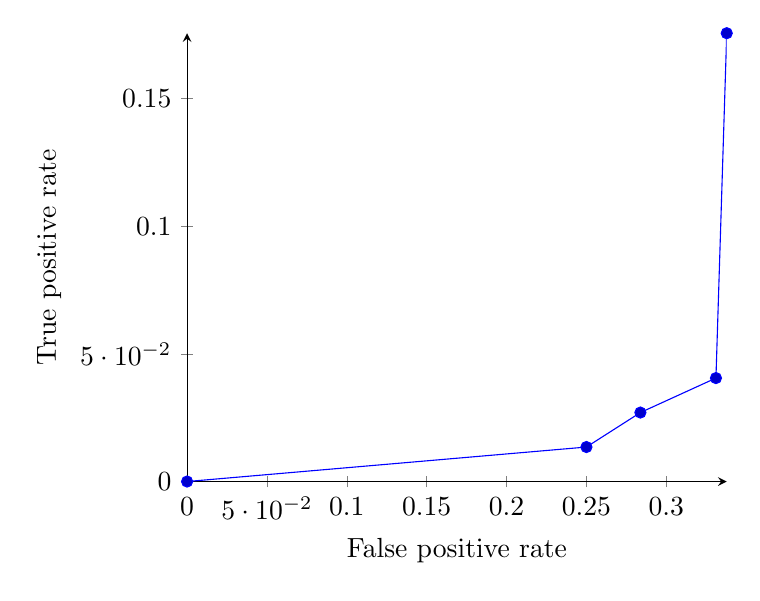
\begin{tikzpicture}
\begin{axis} [xlabel=False positive rate,
ylabel=True positive rate,axis x line=bottom,
axis y line=left]
\addplot coordinates { (0,0)(0.24999999999999978,0.013513513513513514)(0.2837837837837835,0.02702702702702703)(0.3310810810810807,0.04054054054054054)(0.33783783783783744,0.17567567567567569) };\end{axis}
\end{tikzpicture}\hfill \break
 AUC:0.005067567567567559
\hfill \break
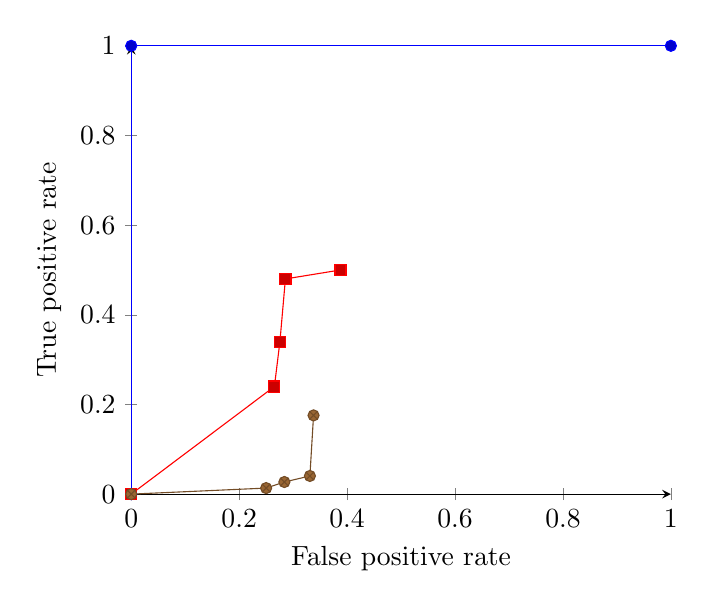
\begin{tikzpicture}
\begin{axis} [xlabel=False positive rate,
ylabel=True positive rate,axis x line=bottom,
axis y line=left]
\addplot coordinates { (0,0)(0,1)(1,1)};
\addplot coordinates { (0,0)(0.2653061224489797,0.23999999999999996)(0.2755102040816328,0.34)(0.28571428571428586,0.48000000000000015)(0.3877551020408166,0.5000000000000001) };
\addplot coordinates { (0,0)(0.24999999999999978,0.013513513513513514)(0.2837837837837835,0.02702702702702703)(0.3310810810810807,0.04054054054054054)(0.33783783783783744,0.17567567567567569) };
\end{axis}
\end{tikzpicture}\hfill \break
File: TRAINING
\hfill \break
\begin{tikzpicture}
\begin{axis} [xlabel=False positive rate,
ylabel=True positive rate,axis x line=bottom,
axis y line=left]
\addplot coordinates { (0,0)(0,1)(1,1)};\end{axis}
\end{tikzpicture}\hfill \break
 AUC:1.0
\hfill \break
\begin{tikzpicture}
\begin{axis} [xlabel=False positive rate,
ylabel=True positive rate,axis x line=bottom,
axis y line=left]
\addplot coordinates { (0,0)(0.2626262626262627,0.2040816326530612) };\end{axis}
\end{tikzpicture}\hfill \break
 AUC:0.02679859822716966
\hfill \break
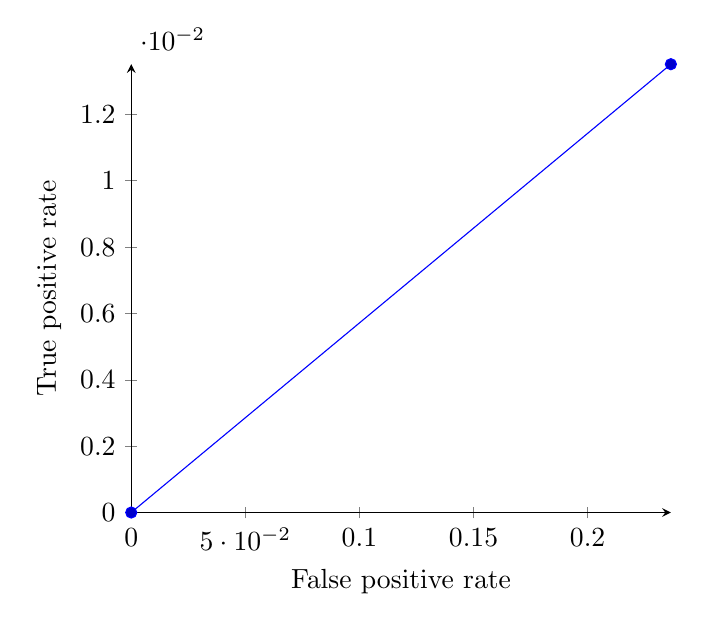
\begin{tikzpicture}
\begin{axis} [xlabel=False positive rate,
ylabel=True positive rate,axis x line=bottom,
axis y line=left]
\addplot coordinates { (0,0)(0.2364864864864863,0.013513513513513514) };\end{axis}
\end{tikzpicture}\hfill \break
 AUC:0.0015978816654492317
\hfill \break
\begin{tikzpicture}
\begin{axis} [xlabel=False positive rate,
ylabel=True positive rate,axis x line=bottom,
axis y line=left]
\addplot coordinates { (0,0)(0,1)(1,1)};
\addplot coordinates { (0,0)(0.2626262626262627,0.2040816326530612) };
\addplot coordinates { (0,0)(0.2364864864864863,0.013513513513513514) };
\end{axis}
\end{tikzpicture}\end{document}